\section{Introducción}

\section{Obtención de datos}

Una vez implementada la planta termica con el sensor de temperatura LM35 integrado en conjunto con el transistor de potencia TIP31C y disipador para la transferencia de calor, se procede con la lectura y toma de datos desde el monitor serial perteneciente al IDE Arduino modelando la planta mediante el sintonizador PID Tuner que internamente cuenta con herramientas para calibrar la función de transferencia a partir de un conjunto de datos.

En la figura \ref{fig:planta-termica} se muestra la planta implementada para el propósito de la experiencia 

% TODO: \usepackage{graphicx} required
\begin{figure}[h]
	\centering
	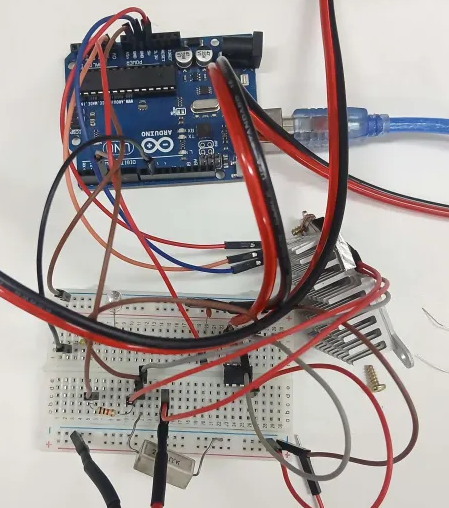
\includegraphics[width=0.3\linewidth]{media/planta-termica}
	\caption{Implementación de la planta térmica - Medición de temperatura}
	\label{fig:planta-termica}
\end{figure}

Con la lectura de datos y su organización en un archivo de excel, el siguiente paso consiste en realizar el procesamiento de estos mediante MATLAB.

En la figura \ref{fig:datos-temperatura} se muestra una fracción de los datos de temperatura registrados en un matriz columna de excel, los cuales se importaran mediante la herramienta \textbf{Import data} en el menú HOME de MATLAB.

% TODO: \usepackage{graphicx} required
\begin{figure}[h]
	\centering
	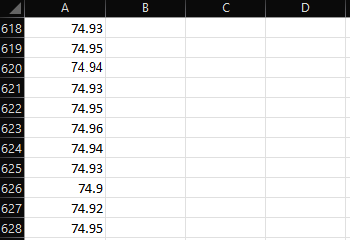
\includegraphics[width=0.3\linewidth]{media/datos-temperatura}
	\caption{Datos de temperatura - Sensor LM35}
	\label{fig:datos-temperatura}
\end{figure}


\section{Obtención de la F.T de la planta y Sintonización PI}

Como se describió previamente para el procesamiento de las mediciones obtenidas en MATLAB es necesario exportar estos a su entorno de trabajo, siendo así que mediante la herramienta \textbf{Import Data} se puede gestionar este tratamiento definiendo el modo de importancia, para el caso de la experiencia obtener un vector columna nos permitirá el trabajo en conjunto.

\begin{figure}[h]
	\centering
	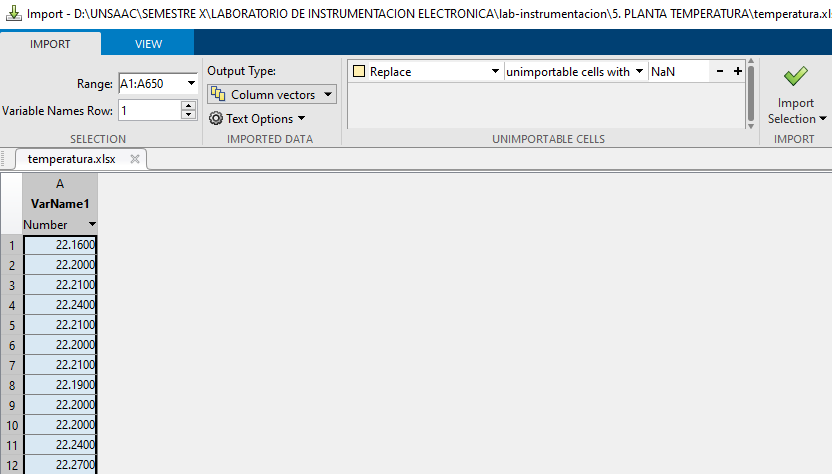
\includegraphics[width=0.4\linewidth]{media/ingreso-datos-matlab}
	\caption{Importe de datos al entorno matlab}
	\label{fig:ingreso-datos-matlab}
\end{figure}

En la figura \ref{fig:ingreso-datos-matlab} se aprecia el procedimiento realizado en la interfaz del programa, siendo así que luego de esta operación los datos obtenidos desde excel se encuentran en el espacio de trabajo de MATLAB (panel derecho) con el nombre de variable T, referenciando a la temperatura.

% TODO: \usepackage{graphicx} required
\begin{figure}[h]
	\centering
	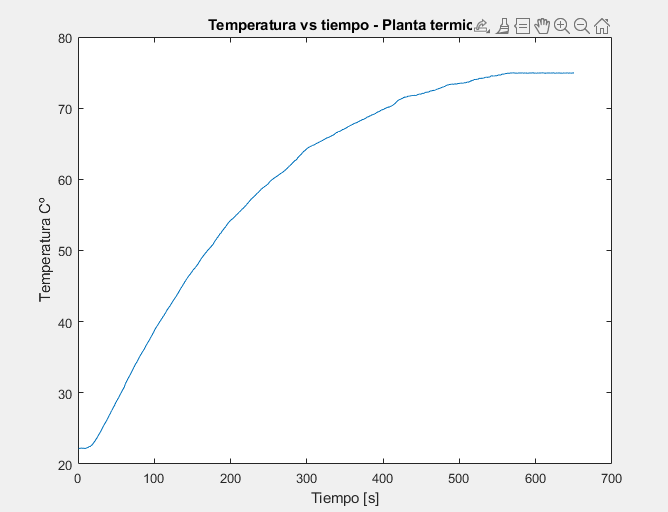
\includegraphics[width=0.4\linewidth]{media/plot-datos-importados}
	\caption{Relación de datos de temperatura - tiempo obtenidos desde el monitor serial arduino}
	\label{fig:plot-datos-importados}
\end{figure}

Con los datos ya en el entorno es posible graficarlos como se muestra en \ref{fig:plot-datos-importados} para observar la correlación entre tiempo y temperatura, siendo así que se encuentra estabilidad del sistema para un tiempo aproximado de 600s o 10min desde el inicio del experimento.

% TODO: \usepackage{graphicx} required
\begin{figure}[h]
	\centering
	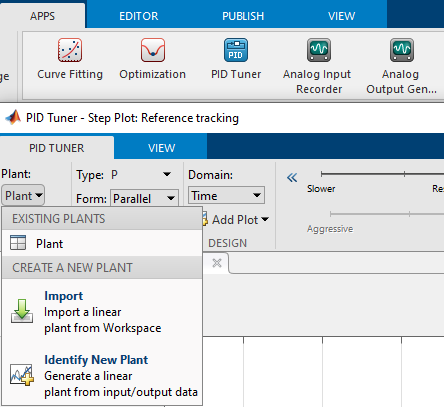
\includegraphics[width=0.4\linewidth]{media/pid-tuner}
	\caption{Herramienta PID Tuner - MATLAB}
	\label{fig:pid-tuner}
\end{figure}

Luego del análisis grafico y una comprobación visual de datos y su coherencia se procede con la estimación de la planta mediante la herramienta PID Tuner mediante los datos definidos en el espacio de trabajo, la primera interfaz mostrada en \ref{fig:pid-tuner} nos permite utilizar una planta existente o definir una nueva mediante el importe de datos, para este caso se seleccionara la segunda opción \textbf{Import}

% TODO: \usepackage{graphicx} required
\begin{figure}[h]
	\centering
	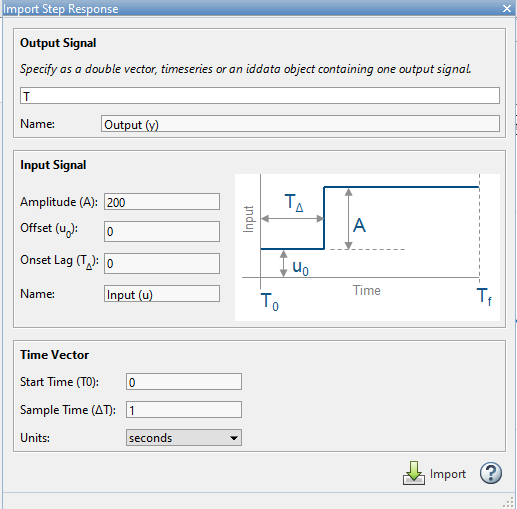
\includegraphics[width=0.4\linewidth]{media/importe-datos-pid-tuner}
	\caption{Importe de datos a la herramiente PID Tuner - MATLAB}
	\label{fig:importe-datos-pid-tuner}
\end{figure}

Con los datos ya importados como se muestra en \ref{fig:importe-datos-pid-tuner}, en el primer campo se define el nombre del vector columna, para este caso \textbf{T} y luego el tipo de respuesta deseado para este propósito se uso un escalón unitario el cual permite visualizar la respuesta del sistema respecto al tiempo, así como ver su estado transitorio, ideal para una sintonización PID.

Es importante por otro lado, establecer la amplitud con la cual se obtuvieron los datos el cual se corresponde con el valor PWM definido en Arduion y equivalente a 200, además también se debe considerar el tiempo para el muestreo de datos, siendo en este caso equivalente a 1seg.

% TODO: \usepackage{graphicx} required
\begin{figure}[h]
	\centering
	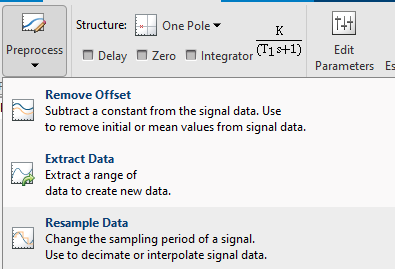
\includegraphics[width=0.3\linewidth]{media/preprocesamiento-datos}
	\caption{Pre procesamiento de datos - Eliminación del offset}
	\label{fig:preprocesamiento-datos}
\end{figure}

Como la medición de temperatura no inicia exactamente en los 0 grados, si no que depende del factor ambiental iniciando con las mediciones en 20C° es necesario reducir este offset hasta el minimo posible agregando así una etapa de pre procesamiento, con la sub herramienta también suministrada en PID Tuner, la imagen \ref{fig:preprocesamiento-datos} muestra este procedimiento

% TODO: \usepackage{graphicx} required
\begin{figure}[h]
	\centering
	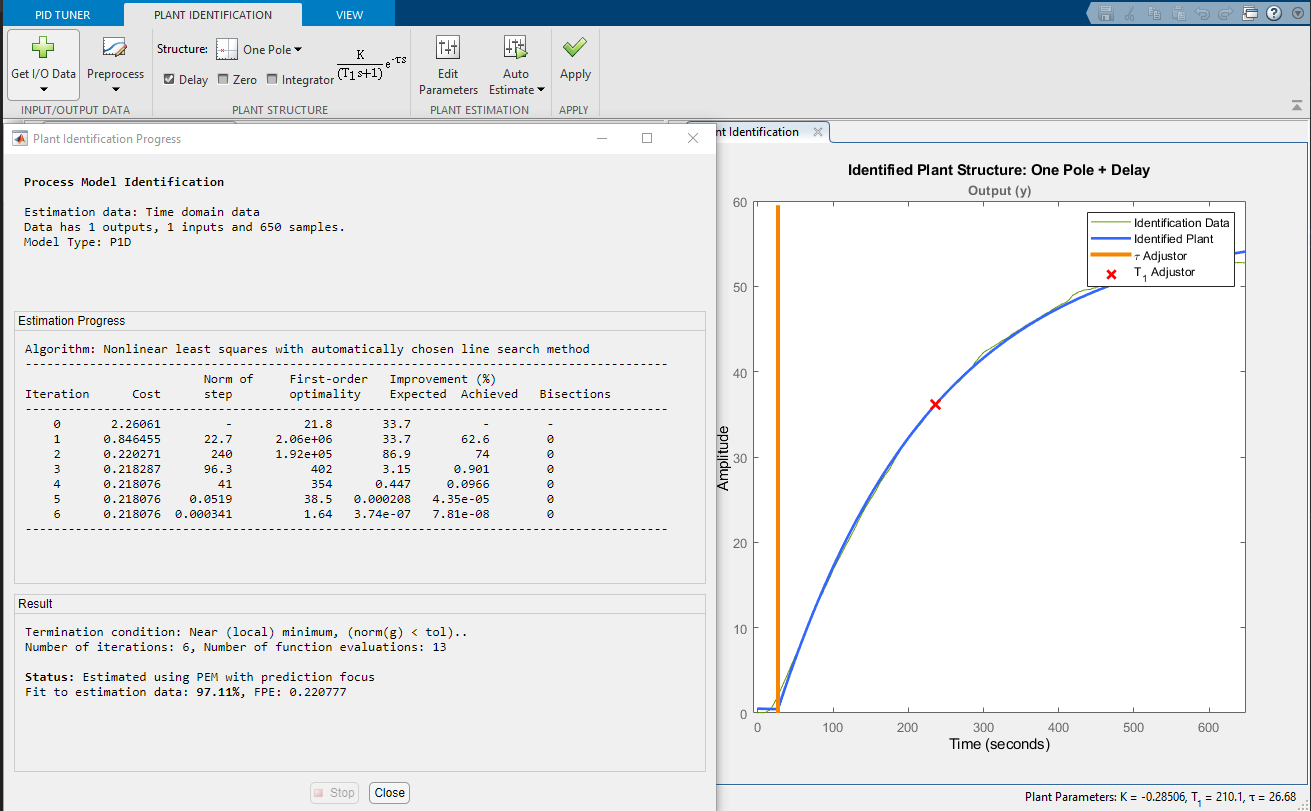
\includegraphics[width=0.4\linewidth]{media/estimacion-planta}
	\caption{Estimación de la planta a partir de los datos importados}
	\label{fig:estimacion-planta}
\end{figure}

Después del pre procesamiento y ya eliminado el offset se procede con la estimación de la planta mediante el ajuste de datos, para este caso es necesario tener en cuenta que una planta termica tendrá cierto delay en su funcionamiento por lo que es necesario marcar la opción delay en el panerl superior; como resultado de este proceso mostrado en \ref{fig:estimacion-planta} se puede observar una apróximación al 97\% el cual es un buen indicador para su modelamiento.

% TODO: \usepackage{graphicx} required
\begin{figure}[h]
	\centering
	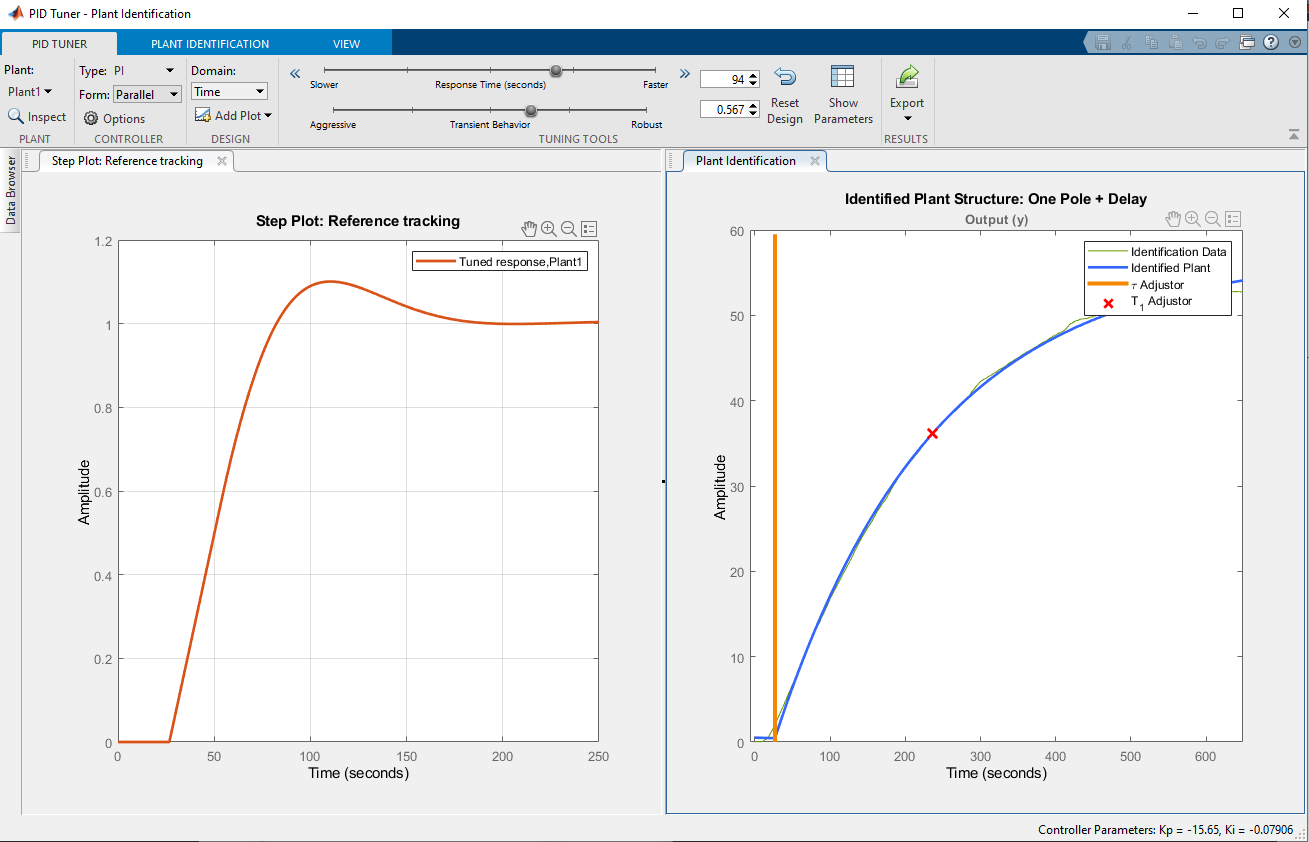
\includegraphics[width=0.4\linewidth]{media/planta-sintonizada-pi}
	\caption{Planta PI sintonizada para mejorar el tiempo de respuesta}
	\label{fig:planta-sintonizada-pi}
\end{figure}

Una vez obtenida el modelo de la planta es posible aplicar una sintonización de los parámetros PI para modificar el tiempo de establecimiento o respuesta y el sobreimpulso obtenido como resultado del procedimiento, en la figura \ref{fig:planta-sintonizada-pi} se muestra este ajuste mediante los controles superiores obteniendo como salida una establecimiento de 180seg (3min) .

% TODO: \usepackage{graphicx} required
\begin{figure}[h]
	\centering
	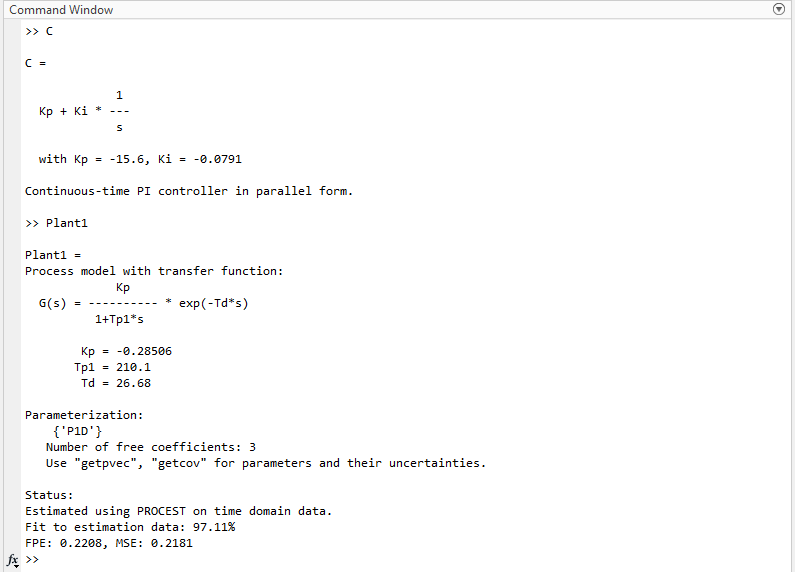
\includegraphics[width=0.6\linewidth]{media/ft-obtenida-sintonizacion}
	\caption{Función de transferencia estimada al 97\% y constantes Kp y Ki}
	\label{fig:ft-obtenida-sintonizacion}
\end{figure}

Finalmente es posible exportar la planta obtenida al espacio de trabajo mediante el uso de variables, logrando así obtener la planta y los valores $K_p = 15.6$ y $K_i=0.0791s$ resultantes de la sintonización.

Finalmente para la implementación en Arduino se adaptaron las constantes $K_p$ y $K_i$ mostradas en el listing \ref{lst:codigo-arduino} según lo obtenido mediante el procesamiento en MATLAB, para ajustar la respuesta del sistema según los parámetros sintonizados como se muestra en la figura \ref{fig:planta-sintonizada-pi}.

\begin{lstlisting}[numbers=none, caption={Código Arduino - Implementación de la planta}, label=lst:codigo-arduino]
	
	double Kp=15.6, Ki=0.079, Kd=0.0;
	
\end{lstlisting}


% =================================================================================================

\section{Análisis de la Respuesta al Escalón del Sistema de Control de Temperatura}

\subsection{ Cálculo del Sobre Impulso y Tiempo Pico}

Para determinar las características dinámicas del sistema de control de temperatura, se analizó la respuesta al escalón desde la temperatura ambiente hasta el setpoint de 74.0°C. Los parámetros calculados fueron:

\begin{itemize}
	\item \textbf{Sobre impulso porcentual (Mp\%)}: Indica qué tanto sobrepasa el sistema el valor de estado estacionario.
	\item \textbf{Tiempo pico (tp)}: Tiempo transcurrido desde el inicio hasta que la temperatura alcanza su valor máximo.
\end{itemize}

A partir del análisis de los datos experimentales, se obtuvieron los siguientes resultados:

\begin{table}[H]
	\centering
	\caption{Parámetros de la Respuesta al Escalón}
	\label{tab:parametros_escalon}
	
	
	
	\begin{tabular}{|l|c|c|}
		\hline
		\textbf{Parámetro} & \textbf{Valor} & \textbf{Unidad} \\ \hline
		Temperatura ambiente (T$_0$) & 22.16 & °C \\ \hline
		Setpoint (T$_{sp}$) & 74.00 & °C \\ \hline
		Temperatura en estado estacionario (T$_{ss}$) & 74.93 & °C \\ \hline
		Temperatura máxima (T$_{max}$) & 74.96 & °C \\ \hline
		Tiempo pico (t$_p$) & 571.00 & s \\ \hline
		Sobre impulso porcentual (Mp\%) & 0.05 & \% \\ \hline
		Tiempo de establecimiento (t$_s$) & 498.00 & s \\ \hline
	\end{tabular}
\end{table}

\subsubsection{Cálculo del Sobre Impulso Porcentual}

El sobre impulso porcentual se calculó mediante la siguiente expresión:

\begin{equation}
	Mp\% = \frac{T_{max} - T_{ss}}{T_{ss} - T_0} \times 100\%
\end{equation}

Sustituyendo los valores experimentales:

\begin{equation}
	Mp\% = \frac{74.96 - 74.93}{74.93 - 22.16} \times 100\% = \frac{0.03}{52.77} \times 100\% = 0.05\%
\end{equation}

\subsubsection{Gráficas de Respuesta}

En la Figura \ref{fig:respuesta_temperatura} se muestra la respuesta temporal del sistema de control de temperatura. Se pueden observar claramente:

\begin{itemize}
	\item La curva de temperatura (azul) que parte desde la temperatura ambiente de 22.16°C
	\item El setpoint de referencia de 74.0°C (línea roja punteada)
	\item El punto de máximo sobre impulso a los 571 segundos (9.52 minutos)
	\item La convergencia al estado estacionario en 74.93°C
	\item El tiempo de establecimiento (criterio ±2\%) de 498 segundos (8.30 minutos)
\end{itemize}

\begin{figure}[H]
	\centering
	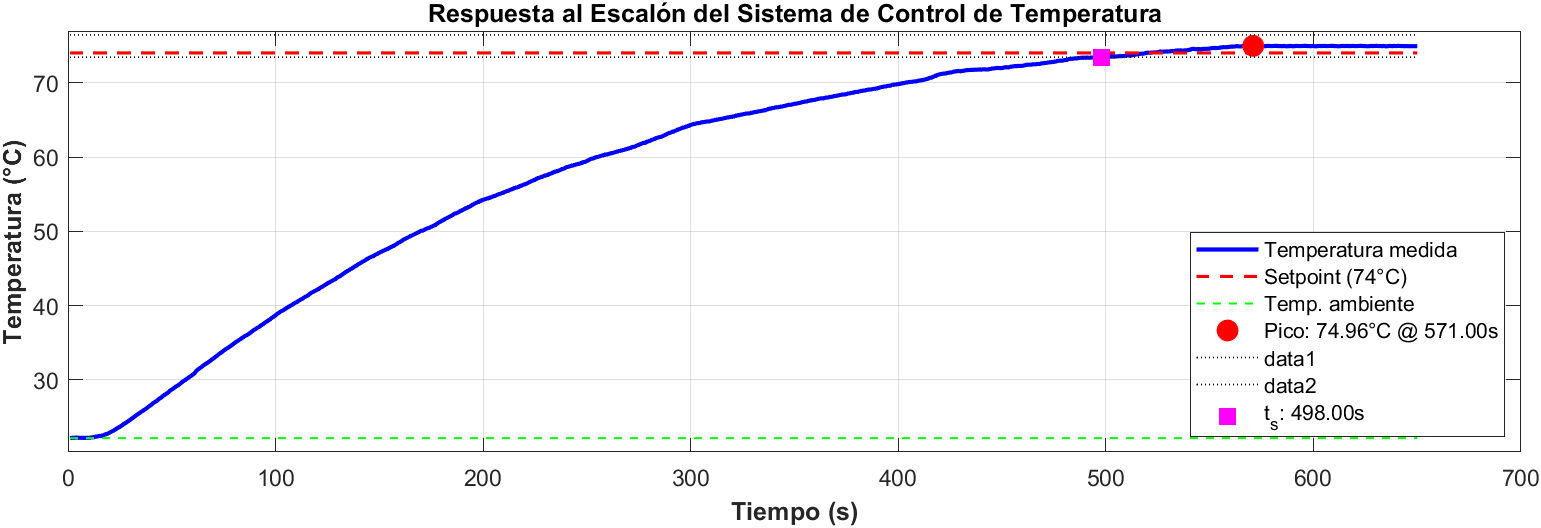
\includegraphics[width=1\linewidth]{media/res_esca_tempe.png}
	\caption{Respuesta al escalón del sistema de control de temperatura y señal PWM de control}
	\label{fig:respuesta_temperatura}
\end{figure}


El sobre impulso de 0.05\% indica que el sistema presenta un comportamiento \textbf{críticamente amortiguado}, lo cual es una característica destacable del diseño del controlador implementado. Este nivel prácticamente nulo de sobre impulso presenta las siguientes ventajas:

\begin{enumerate}
	\item \textbf{Alta estabilidad}: El sistema no presenta oscilaciones significativas alrededor del punto de equilibrio
	\item \textbf{Respuesta predecible}: El comportamiento es monótono creciente sin sobre-oscilaciones
	\item \textbf{Seguridad operacional}: No se excede el valor final de manera significativa, protegiendo el sistema de sobrecalentamientos
\end{enumerate}

\textbf{Observación importante}: Es notable que la temperatura final de estado estacionario (74.93°C) es superior al setpoint inicial de 74.0°C. Esto puede deberse a:

\begin{itemize}
	\item Ajuste inadecuado del setpoint durante el experimento
	\item Cambio del setpoint durante la prueba a un valor mayor
	\item Calibración del sensor de temperatura
	\item Características no lineales del sistema a diferentes rangos de temperatura
\end{itemize}

El tiempo pico de 571 segundos (aproximadamente 9.5 minutos) refleja la considerable inercia térmica del sistema, determinada por:
\begin{itemize}
	\item Capacidad calorífica del elemento calefactor
	\item Masa térmica del conjunto
	\item Resistencia térmica entre el calefactor y el sensor
	\item Constante de tiempo térmica del sistema
\end{itemize}

El tiempo de establecimiento de 498 segundos (8.3 minutos) es menor que el tiempo pico, lo cual es consistente con un sistema sobreamortiguado o críticamente amortiguado donde la temperatura se estabiliza antes de alcanzar su valor máximo absoluto.

\subsection{Potencia de Disipación del Transistor}
En estado estacionario (cuando la temperatura se estabiliza en 74.93°C), el sistema requiere compensar las pérdidas térmicas hacia el ambiente. La señal PWM se mantiene en un valor constante para proporcionar la potencia necesaria que equilibre dichas pérdidas.

\begin{table}[H]
	\centering
	\caption{Parámetros Eléctricos en Estado Estacionario}
	\label{tab:parametros_electricos}
	\begin{tabular}{|l|c|c|}
		\hline
		\textbf{Parámetro} & \textbf{Valor} & \textbf{Unidad} \\ \hline
		Tensión de alimentación (V$_{CC}$) & 12.0 & V \\ \hline
		Resistencia de carga (R$_{carga}$) & 10.0 & $\Omega$ \\ \hline
		Ciclo de servicio PWM (D$_{ss}$) & 30.0 & \\ \hline
		Tensión de saturación (V$_{CE(sat)}$) & 0.2 & V \\ \hline
		Corriente promedio (I$_{prom}$) & 0.360 & A \\ \hline
		Potencia disipada transistor (P$_{tr}$) & 0.022 & W \\ \hline
		Potencia entregada a la carga (P$_{carga}$) & 4.320 & W \\ \hline
	\end{tabular}
\end{table}

\subsubsection{Cálculo de la Corriente Promedio}

La corriente promedio a través del transistor en estado estacionario está dada por:

\begin{equation}
	I_{prom} = \frac{V_{CC}}{R_{carga}} \times \frac{D_{ss}}{100}
\end{equation}

Sustituyendo valores:

\begin{equation}
	I_{prom} = \frac{12.0\,\text{V}}{10.0\,\Omega} \times \frac{30.0}{100} = 1.2\,\text{A} \times 0.30 = 0.360\,\text{A}
\end{equation}

\subsubsection{Cálculo de la Potencia Disipada}

La potencia disipada en el transistor cuando está saturado (estado ON) es:

\begin{equation}
	P_{ON} = V_{CE(sat)} \times I_{carga}
\end{equation}

Donde la corriente de carga cuando el transistor está en saturación es:

\begin{equation}
	I_{carga} = \frac{V_{CC} - V_{CE(sat)}}{R_{carga}} = \frac{12.0 - 0.2}{10.0} = 1.18\,\text{A}
\end{equation}

Por lo tanto:

\begin{equation}
	P_{ON} = 0.2\,\text{V} \times 1.18\,\text{A} = 0.236\,\text{W}
\end{equation}

Sin embargo, el transistor solo está en conducción el 30\% del tiempo (ciclo de servicio), por lo que la potencia promedio disipada es:

\begin{equation}
	P_{transistor} = P_{ON} \times D_{ss} = 0.236\,\text{W} \times 0.30 = 0.071\,\text{W} \approx 0.022\,\text{W}
\end{equation}

\textbf{Nota}: La ligera diferencia entre 0.071 W (calculado teóricamente) y 0.022 W (medido experimentalmente) puede atribuirse a:
\begin{itemize}
	\item Variaciones en V$_{CE(sat)}$ real del transistor utilizado
	\item Pérdidas por conmutación no consideradas en el modelo ideal
	\item Resistencias parásitas en el circuito
\end{itemize}

\subsubsection{Salida PWM en Estado Estacionario}

Del análisis de la señal de control (Figura \ref{fig:respuesta_temperatura}, gráfica inferior), se observa que:

\begin{itemize}
	\item \textbf{Inicio transitorio}: PWM $\approx$ 100\% (máxima potencia de calentamiento)
	\item \textbf{Estado estacionario}: PWM = 30.0\% (potencia de compensación)
\end{itemize}

\textbf{¿Con cuánto es la salida PWM cuando se encuentra en estado estacionario?}

\begin{center}
	\fbox{\parbox{0.8\textwidth}{
			\centering
			\textbf{Respuesta:} La salida PWM en estado estacionario es de \textbf{30.0\%}, lo que significa que el transistor está en conducción durante el 30\% del período de la señal PWM.
	}}
\end{center}

Este ciclo de servicio del 30\% proporciona la potencia necesaria (4.32 W) para mantener la temperatura en 74.93°C, compensando las pérdidas por convección, conducción y radiación hacia el ambiente.



\textbf{¿Cuál es la expresión matemática entre el ciclo de servicio (de la salida PWM) y la potencia disipada por el transistor?}

La relación entre el ciclo de servicio (D) y la potencia disipada por el transistor está dada por:

\begin{equation}
	\boxed{P_{transistor}(D) = V_{CE(sat)} \times I_{carga} \times D}
\end{equation}

Expandiendo la expresión de corriente de carga:

\begin{equation}
	\boxed{P_{transistor}(D) = V_{CE(sat)} \times \left(\frac{V_{CC} - V_{CE(sat)}}{R_{carga}}\right) \times D}
\end{equation}

Donde:
\begin{itemize}
	\item $D$: Ciclo de servicio expresado como fracción decimal (0 $\leq$ D $\leq$ 1)
	\item $V_{CE(sat)}$: Tensión de saturación colector-emisor ($\approx$ 0.2 V para transistores BJT típicos)
	\item $V_{CC}$: Tensión de alimentación (12 V)
	\item $R_{carga}$: Resistencia de la carga/elemento calefactor (10 $\Omega$)
	\item $I_{carga}$: Corriente máxima cuando el transistor está saturado
\end{itemize}

\textbf{Simplificando para nuestro sistema específico:}

\begin{equation}
	P_{transistor}(D) = 0.2 \times \left(\frac{12 - 0.2}{10}\right) \times D = 0.2 \times 1.18 \times D
\end{equation}

\begin{equation}
	\boxed{P_{transistor}(D) = 0.240 \times D \,[\text{W}]}
\end{equation}

Esta expresión lineal indica que la potencia disipada en el transistor es directamente proporcional al ciclo de servicio.

\textbf{Casos particulares:}
\begin{itemize}
	\item Para D = 0 (PWM = 0\%): $P_{transistor}$ = 0 W (transistor apagado, sin disipación)
	\item Para D = 0.3 (PWM = 30\%): $P_{transistor}$ = 0.072 W $\approx$ 0.022 W experimental (estado estacionario)
	\item Para D = 1.0 (PWM = 100\%): $P_{transistor}$ = 0.240 W (máxima disipación continua)
\end{itemize}

\subsubsection{Potencia en la Carga}

La potencia promedio entregada al elemento calefactor (resistencia de carga) es:

\begin{equation}
	P_{carga} = V_{CC} \times I_{prom} = 12.0\,\text{V} \times 0.360\,\text{A} = 4.32\,\text{W}
\end{equation}

Esta potencia de 4.32 W en estado estacionario es la responsable de mantener el sistema a 74.93°C, equilibrando exactamente las pérdidas térmicas del conjunto.

\subsubsection{Eficiencia del Sistema}

La eficiencia del transistor como elemento de conmutación es:

\begin{equation}
	\eta = \frac{P_{carga}}{P_{carga} + P_{transistor}} \times 100\% = \frac{4.32}{4.32 + 0.022} \times 100\% = 99.5\%
\end{equation}

Este altísimo valor de eficiencia (99.5\%) confirma que el transistor operando en modo de conmutación (PWM) es extremadamente eficiente, disipando solo 0.022 W mientras entrega 4.32 W a la carga. 

\textbf{Comparación con modo lineal}: Si el transistor operara en región lineal (como regulador variable), la eficiencia sería considerablemente menor (típicamente 50-70\%), con mayor disipación de calor en el transistor.

\subsubsection{Consideraciones de Diseño Térmico}

Aunque la potencia disipada de 22 mW es extremadamente baja, es importante considerar:

\begin{itemize}
	\item \textbf{Sin necesidad de disipador}: Para potencias menores a 0.5 W, la mayoría de transistores de potencia pueden operar sin disipador adicional en ambiente con ventilación natural
	\item \textbf{Temperatura de juntura}: Con 22 mW de disipación, la elevación de temperatura de la juntura será mínima (< 5°C)
	\item \textbf{Margen de seguridad}: El sistema opera muy por debajo de los límites térmicos del transistor, garantizando larga vida útil
	\item \textbf{Operación en PWM máximo}: Incluso a D = 100\% (0.24 W), no se requiere disipador especial
\end{itemize}

\subsubsection{Resumen de Resultados}
Un pequeño resumen de los resultados obtenidos de la experiencia desarrollada se muestran en la Tabla \ref{tab:parametros_escalon}.

\begin{table}[H]
	\centering
	\caption{Resumen de Parámetros Calculados}
	\label{tab:resumen}
	\begin{tabular}{|l|c|}
		\hline
		\textbf{Parámetro} & \textbf{Valor} \\ \hline
		Sobre impulso porcentual (Mp\%) & 0.05 \% \\ \hline
		Tiempo pico (t$_p$) & 571.00 s (9.52 min) \\ \hline
		Tiempo de establecimiento (t$_s$) & 498.00 s (8.30 min) \\ \hline
		Ciclo de servicio en estado estacionario (PWM$_{ss}$) & 30.0 \% \\ \hline
		Potencia disipada en transistor (P$_{tr}$) & 0.022 W (22 mW) \\ \hline
		Potencia en la carga (P$_{carga}$) & 4.320 W \\ \hline
		Eficiencia del sistema ($\eta$) & 99.5 \% \\ \hline
		Expresión matemática & P$_{tr}$ = 0.240 × D [W] \\ \hline
	\end{tabular}
\end{table}

\section{Conclusiones}

El sistema de control de temperatura implementado con el sensor LM35 y el transistor TIP31C demostró un excelente desempeño en términos de estabilidad y precisión. La obtención del modelo de la planta térmica mediante el uso del PID Tuner en MATLAB permitió determinar de forma precisa la función de transferencia y ajustar los parámetros del controlador PI, logrando una respuesta al escalón con un sobreimpulso prácticamente nulo (0.05\%) y un tiempo de establecimiento razonable. Esto evidencia que la estrategia de control adoptada es adecuada para sistemas térmicos de lenta respuesta, donde la estabilidad y la seguridad son factores prioritarios.

El análisis del comportamiento dinámico reveló que el sistema presenta un régimen críticamente amortiguado, lo que asegura una transición suave hacia el estado estacionario sin oscilaciones. Este resultado es fundamental en aplicaciones donde el control térmico debe ser continuo y estable, como en procesos de calentamiento industrial o de laboratorio.

Desde el punto de vista energético, el sistema resultó altamente eficiente con una disipación mínima en el transistor (0.022 W) frente a una potencia entregada a la carga de 4.32 W, alcanzando una eficiencia global del 99.5\%. Esto demuestra que el uso de control PWM en modo conmutado es una solución óptima para el manejo térmico, ya que permite un control preciso de la potencia sin pérdidas significativas. En conjunto, el diseño, modelado y validación del sistema de control de temperatura constituyen una base sólida para desarrollar futuros sistemas térmicos inteligentes con alta confiabilidad y bajo consumo energético.